\documentclass[a4paper,12pt]{article}

%%% Работа с русским языком
\usepackage{cmap}					% поиск в PDF
\usepackage{mathtext} 				% русские буквы в формулах
\usepackage[T2A]{fontenc}			% кодировка
\usepackage[utf8]{inputenc}			% кодировка исходного текста
\usepackage[english,russian]{babel}	% локализация и переносы
\usepackage{xcolor}
\usepackage{hyperref}
 % Цвета для гиперссылок
\definecolor{linkcolor}{HTML}{799B03} % цвет ссылок
\definecolor{urlcolor}{HTML}{799B03} % цвет гиперссылок

\hypersetup{pdfstartview=FitH,  linkcolor=linkcolor,urlcolor=urlcolor, colorlinks=true}

%%% Дополнительная работа с математикой
\usepackage{amsfonts,amssymb,amsthm,mathtools} % AMS
\usepackage{amsmath}
\usepackage{icomma} % "Умная" запятая: $0,2$ --- число, $0, 2$ --- перечисление

%% Номера формул
%\mathtoolsset{showonlyrefs=true} % Показывать номера только у тех формул, на которые есть \eqref{} в тексте.

%% Шрифты
\usepackage{euscript}	 % Шрифт Евклид
\usepackage{mathrsfs} % Красивый матшрифт

%% Свои команды
\DeclareMathOperator{\sgn}{\mathop{sgn}}

%% Перенос знаков в формулах (по Львовскому)
\newcommand*{\hm}[1]{#1\nobreak\discretionary{}
{\hbox{$\mathsurround=0pt #1$}}{}}
% графика
\usepackage{graphicx}
\graphicspath{{pictures/}}
\DeclareGraphicsExtensions{.pdf,.png,.jpg}
\author{Бурмашев Григорий, БПМИ-208}
\title{Матан, дз -- 11?}
\date{\today}
\begin{document}
\section*{Номер 1}
\subsection*{a)}
\[
1 \leq | z + 2 + i | \leq 2
\]	
По аналогии с семинаром замечаем, что это будет окружность с центром в точке $(-2, -1)$. А ограничение с двух сторон будет задавать некий бублик (Для $\leq 2$ берем всё внутри окружности радиуса 2, для $\geq 1$ берем всё снаружи окружности радиуса 1, вот и получается бублик). На графике это будет иметь вид:
\begin{center}
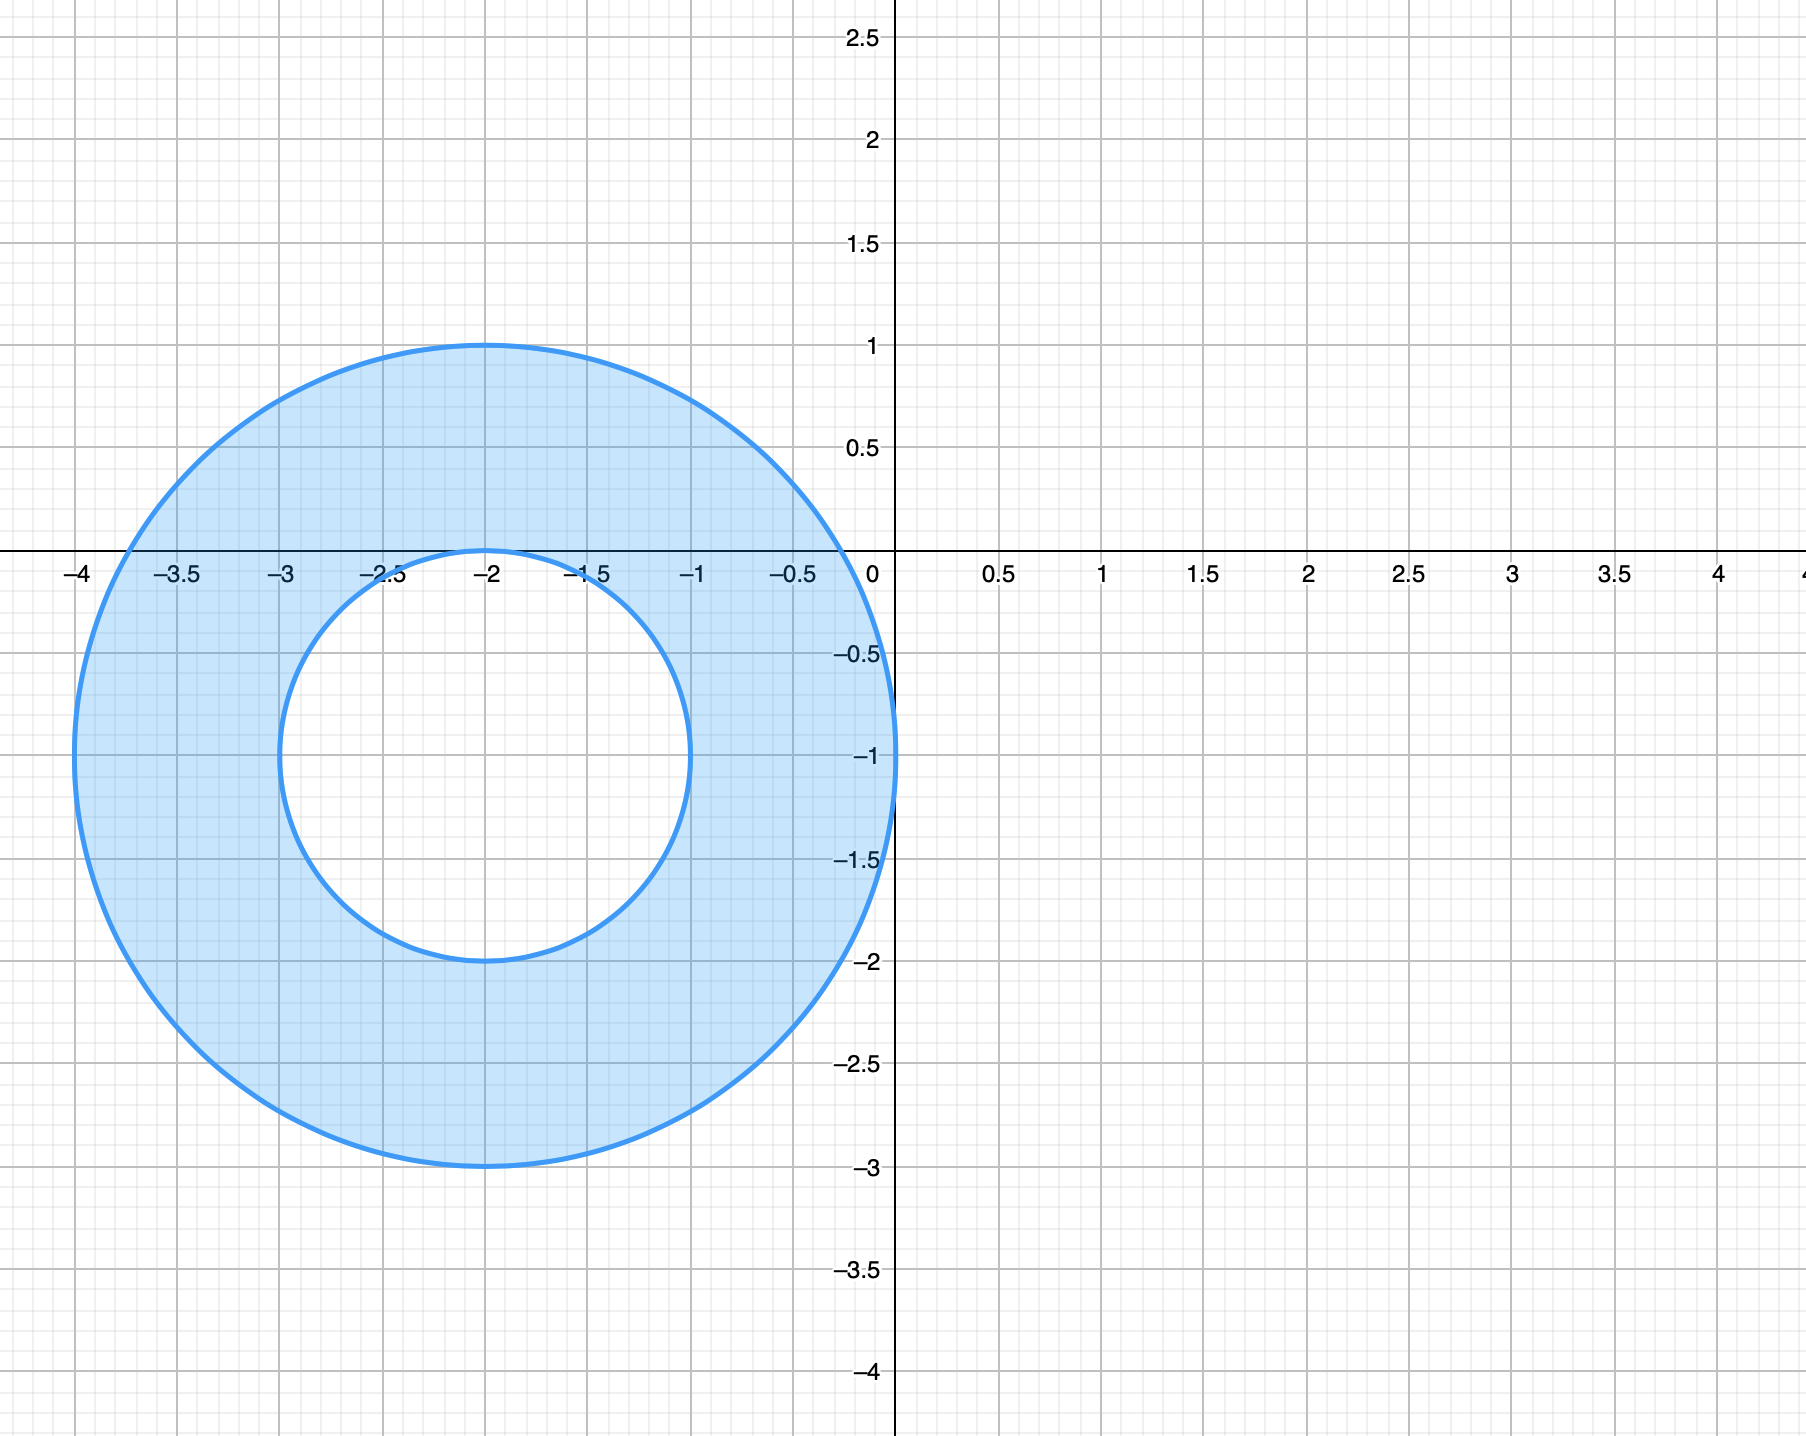
\includegraphics[scale=0.3]{1.png}
\end{center}
\clearpage
\subsection*{b)}
\[
|\pi - \arg z | < \frac{\pi}{4}
\]
Избавимся от модуля:
\[
- \frac{\pi}{4} < \pi - \arg z  < \frac{\pi}{4}
\]
\[
- \frac{\pi}{4} < \pi - \arg z  < \frac{\pi}{4}
\]
\[
- \frac{5\pi}{4} < - \arg z  < -\frac{3\pi}{4}
\]
\[
\frac{3\pi}{4} <  \arg z  < \frac{5\pi}{4}
\]
Получаем график (нам подходит все, что зажато между двумя прямыми, образованными $\arg(z)$):
\begin{center}
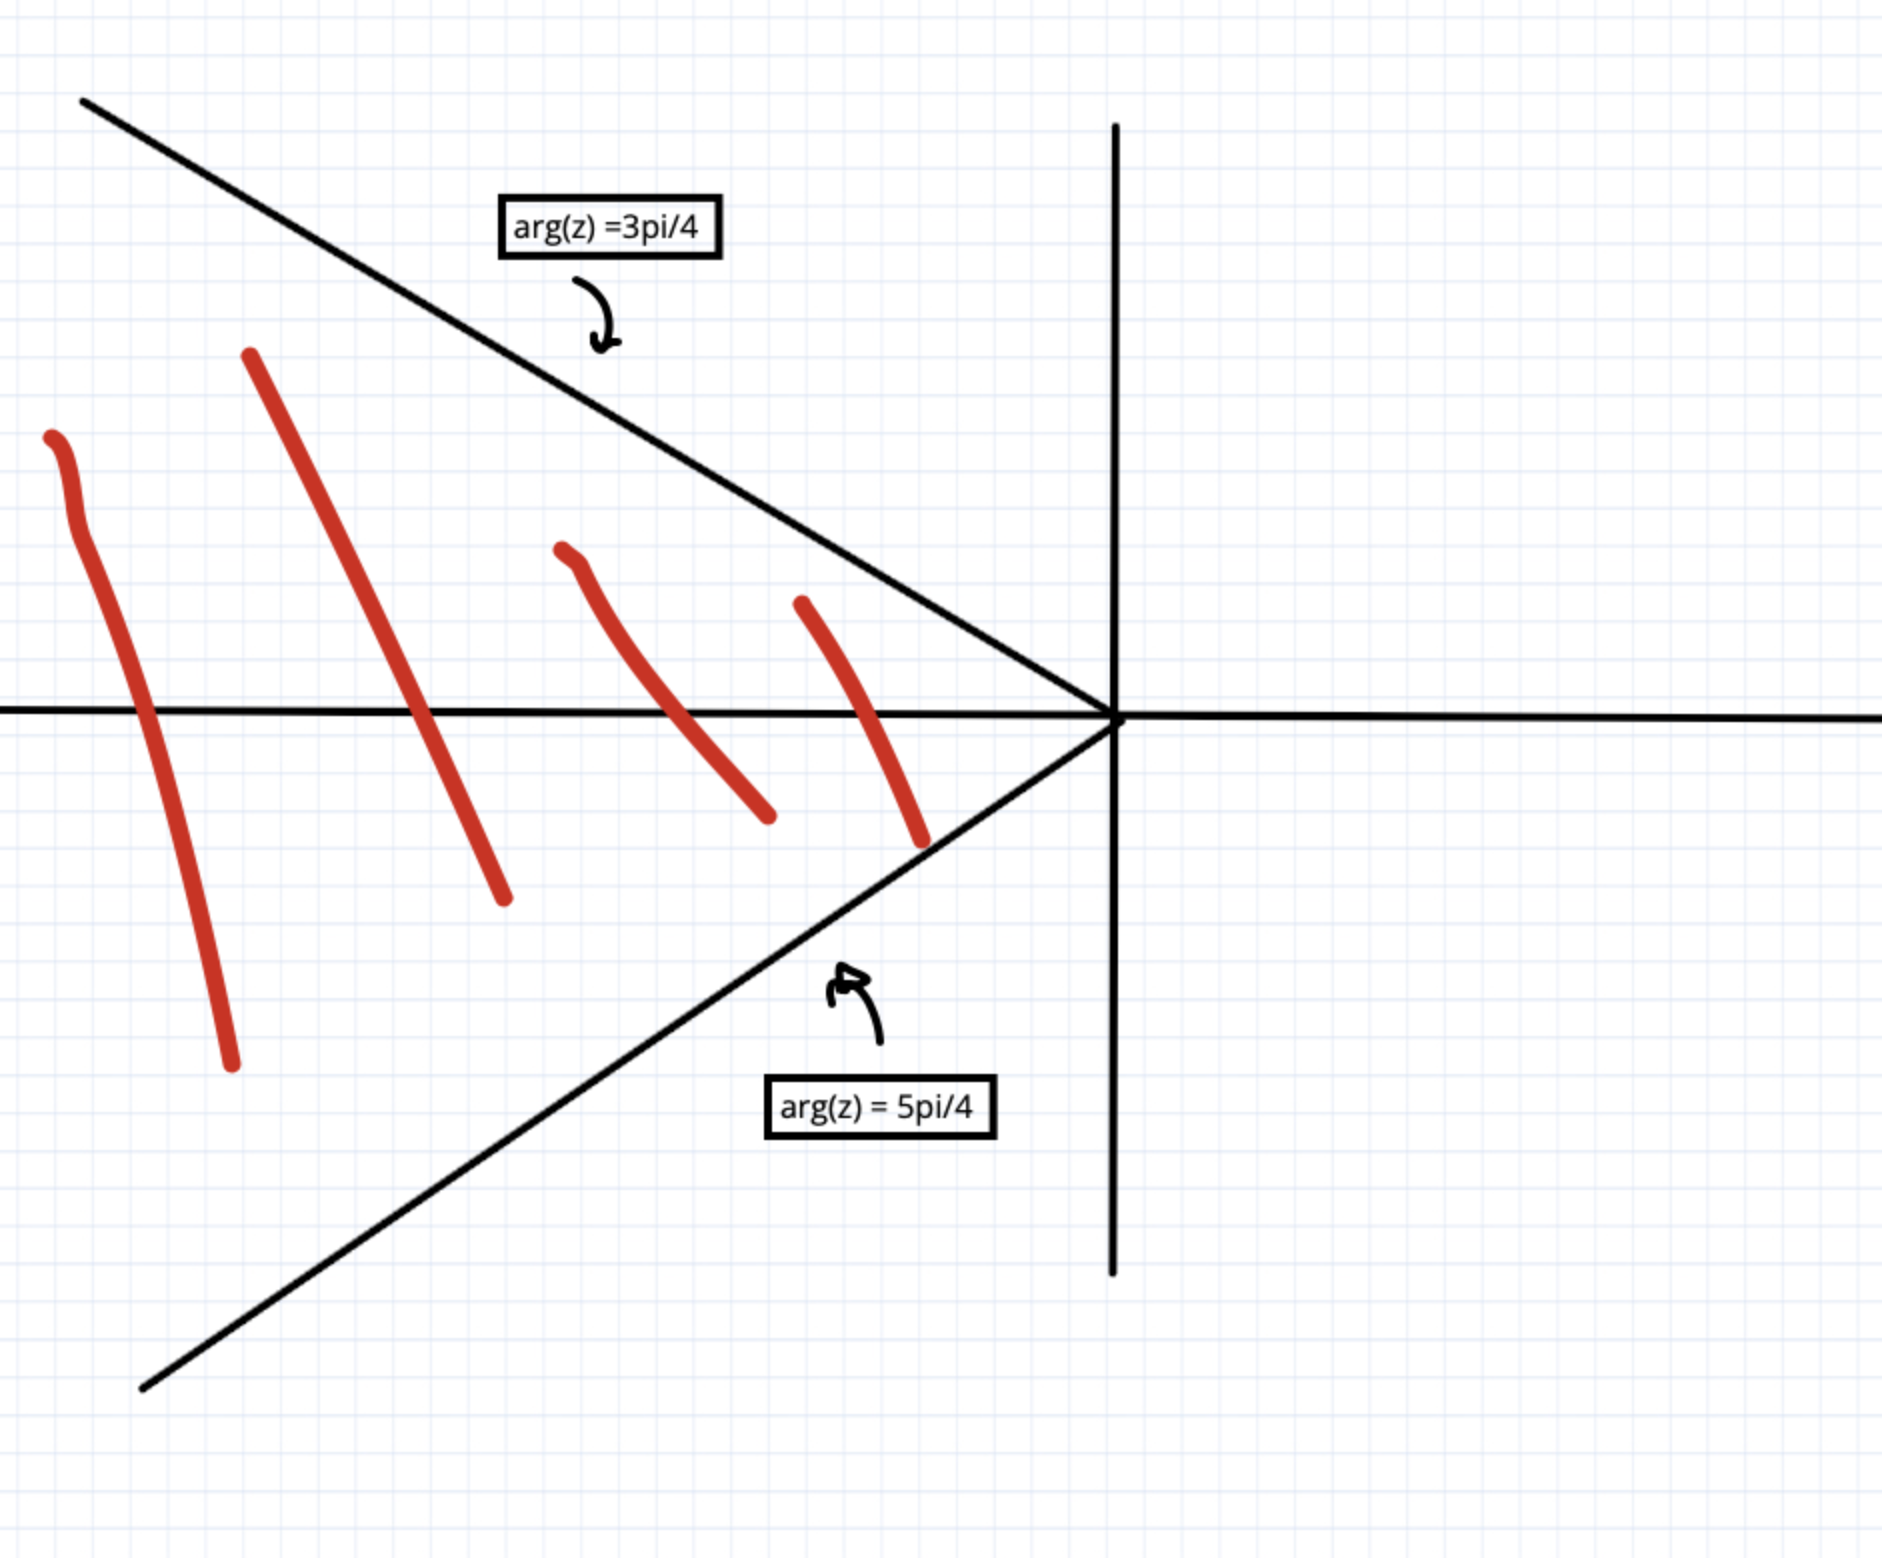
\includegraphics[scale=0.3]{2.png}
\end{center}
\clearpage
\section*{Номер 2}
\subsection*{a)}
\[
Ln (z) - Ln(z) = 0 ?
\]
Знаем свойство:
\[
Ln \left(\frac{z_1}{z_2}\right) = Ln(z_1) - Ln(z_2) 
\]
Применяем его в нашем случае и получаем:
\[
Ln (z) - Ln(z)  = Ln \left(\frac{z}{z}\right) = Ln(1) = 2k \pi i 
\]
Видим, что оно не равно нулю при всех $k$, отличных от нуля, значит утверждение неверное
\begin{center}
\textbf{Ответ: } нет, неверно  
\end{center}
\subsection*{b)}
\[
\sin (2z) = 2 \sin z \cos z ?
\]
Подставим по определению:
\[
\sin (2z) = \frac{e^{i2z} \cdot e^{-i2z}}{2i}
\]
\[
2 \sin z \cos z  = 2 \cdot \frac{e^{iz} \cdot e^{-iz}}{2i} \cdot \frac{e^{iz} +  e^{-iz}}{2} =  \frac{e^{iz + iz} - e^{-iz - iz}}{2i} = \frac{e^{i2z} \cdot e^{-i2z}}{2i}
\]
Получаем равенство
\begin{center}
\textbf{Ответ: } да, верно
\end{center}
\clearpage
\section*{Номер 3}
\[
\sin z - \cos z = i
\]
Подставляем по определению:
\[
\frac{e^{iz} - e^{-iz}}{2i} - \frac{e^{iz} + e^{-iz}}{2} = i
\]
Умножаем на $e^{iz}$ обе части:
\[
\frac{e^{2iz} - e^{0}}{2i} - \frac{e^{2iz} + e^{0}}{2} = e^{iz}i
\]
\[
\frac{e^{2iz} - 1}{2i} - \frac{e^{2iz} + 1}{2} = e^{iz}i
\]
\[
\frac{e^{2iz} - 1}{2} - \frac{i(e^{2iz} + 1)}{2} = -e^{iz}
\]
\[
e^{2iz} - 1- i(e^{2iz} + 1) = -2e^{iz}
\]
\[
e^{2iz} - 1- i(e^{2iz} + 1)  + 2e^{iz} = 0
\]
\[
e^{2iz}(1 - i) + 2e^{iz} - 1 - i = 0
\]
Считаем дискриминант:
\[
D = 2^2 - 4 \cdot (1 - i) (-1 - i) = 12 
\]
Тогда:
\[
e^{iz} = \frac{-2 \pm  \sqrt{12}}{2(1 - i)} = \frac{-1 \pm \sqrt{3}}{1- i} = \frac{(-1 \pm \sqrt{3})(1 + i)}{2}  =\frac{(1 + i)}{2}(-1 \pm \sqrt{3}) =  \frac{(-1 \pm \sqrt{3})\sqrt{2}e^{i \frac{\pi}{4}}}{2}  =
\]
\[
=
\frac{(-1 \pm \sqrt{3})e^{i \frac{\pi}{4}}}{\sqrt{2}}  
\]
Очень хочется сделать как на семинаре и в тупую внести все под $e$, но там вылезает отрицательное число внутри логарифма (я не особо шарю и не хочу лезть в комплексные логарифмы), так что посмотрим отдельно на два случая и избавимся от минуса, чтобы нормально внести:
\[
e^{iz} = 
\left[ 
      \begin{gathered} 
        \frac{(-1 +  \sqrt{3})}{\sqrt{2}}  e^{i \frac{\pi}{4}}\\
	  \frac{(-1 -  \sqrt{3})}{\sqrt{2}} e^{i \frac{\pi}{4}}
      \end{gathered} 
\right.
\]
\[
e^{iz} = 
\left[ 
      \begin{gathered} 
        e^{\ln \left( \frac{(-1 +  \sqrt{3})}{\sqrt{2}}  \right) } e^{i \frac{\pi}{4}}\\
	  \frac{-1(1 +  \sqrt{3})}{\sqrt{2}} e^{i \frac{\pi}{4}}
      \end{gathered} 
\right.
\]
\[
e^{iz} = 
\left[ 
      \begin{gathered} 
        e^{\ln \left( \frac{(-1 +  \sqrt{3})}{\sqrt{2}}  \right) } e^{i \frac{\pi}{4}}\\
	  e^{i \pi }e^{\ln \left( \frac{(1 +  \sqrt{3})}{\sqrt{2}}\right)}e^{i \frac{\pi}{4}}
      \end{gathered} 
\right.
\]
\[
e^{iz} = 
\left[ 
      \begin{gathered} 
        e^{\ln \left( \frac{(-1 +  \sqrt{3})}{\sqrt{2}}  \right)  + i \frac{\pi}{4}} \\
	  e^{\ln \left( \frac{(1 +  \sqrt{3})}{\sqrt{2}}\right) + i \pi + i \frac{\pi}{4} }
      \end{gathered} 
\right.
\]
Отсюда:
\[
z = 
\left[ 
      \begin{gathered} 
       -i \ln \left(
	\frac{-1 + \sqrt{3}}{\sqrt{2}} \right) + \frac{\pi}{4} + 2 \pi k \\
	-i \ln \left(
	\frac{1 + \sqrt{3}}{\sqrt{2}} \right) + \frac{5\pi}{4} + 2 \pi k 
      \end{gathered} 
\right.
\]
\begin{center}
\textbf{Ответ: } 
\[
z = 
\left[ 
      \begin{gathered} 
       -i \ln \left(
	\frac{-1 + \sqrt{3}}{\sqrt{2}} \right) + \frac{\pi}{4} + 2 \pi k \\
	-i \ln \left(
	\frac{1 + \sqrt{3}}{\sqrt{2}} \right) + \frac{5\pi}{4} + 2 \pi k 
      \end{gathered} 
\right.
\]
\end{center}
\clearpage
\section*{Номер 4}
Замечаем:
\[
z^2 = x^2 + 2ixy - y^2
\]
Назовем $x = c_1$, тогда:
\[
\begin{cases}
u = Re \;w = c_1^2 - y^2 \\
v = Im\;  w =2 c_1 y
\end{cases}
\]
\[
\begin{cases}
u = c_1^2 - \frac{v^2}{4c_1^2} \\
y = \frac{v}{2c_1}
\end{cases}
\]
Видим, что это параболка.
Назовем $y = c_2$, тогда:
\[
\begin{cases}
u = x^2 - c_2^2 \\
v = 2c_ 2 x
\end{cases}
\]
\[
\begin{cases}
u = \frac{v^2}{4c_2^2} - c_2^2 \\
x = \frac{v}{2c_2}
\end{cases}
\]
Видим, что это снова параболка. Значит прямые переходят в параболы
\begin{center}
\textbf{Ответ: } переходят в параболы
\end{center}
\end{document}
